\chapter{АНАЛИТИЧЕСКИЙ РАЗДЕЛ}
В разных разделах этой главы он использует отзывы пользователей, чтобы принимать решения об изменении при представлении предложений. Как читать эту главу: В разделе 1.1 представлена функциональная схема системы: типичный системный модуль рекомендации, модуль управления новыми идеями для совместной экономики и развития района и города.

В разделе 1.2 приводится краткий обзор того, какая система рекомендаций по использованию и приобретению товаров и услуг для домашнего благоустройства, выставок и культурных мероприятий. Математическая формулировка и показатели, доступные для оценки производительности.

В разделе 1.3 сначала анализируется подход «Совместная фильтрация», в котором подчеркиваются его характеристики, сильные и слабые стороны, и таким же образом с подходом, основанным на содержании, один из двух будет принят.

В разделе 1.4 анализируются альтернативы, которые возникают в результате улучшений, применяемых к районам, по сравнению с более развитыми в данной области, а также возможности для улучшения с точки зрения лучшего предложения или с учетом рекомендаций раздела 1.5 о совместной экономике и краудсорсинге через вклад жителей. Наконец, разделы 1.6 и 1.7 касаются модуля отчетов о проблемах города, в которых жители сообщают об инцидентах, и идеи, которые они могут внести в интересах развития города.


\section{Функциональная схема модели}
Выделяется модуль типичной системы рекомендаций, модуль управления новыми идеями для совместной экономики и развития района и города.

Поиск способов улучшения жилых районов начинается с анализа привычек потребления групп, проживающих в определенных городских анклавах, в соответствии с сбором информации из системы рекомендаций по купле-продаже по двум конкретным предметам. Первая группа занимается предметами благоустройства дома: садово-парковые изделия, растения и цветы, картины для дома и мебели. В то время как вторая касается предложений культурной и развлекательной деятельности.

Впоследствии оцениваются степень эволюции данного района как взвешивания суммы всего движения или деятельности как группы, а сравнения с другими соседями проводятся с целью внесения изменений или предложений по улучшению.

Впоследствии оцениваются степень эволюции данного района как взвешивания суммы всего движения или деятельности в качестве группы, и проводится сравнение с другими районами с целью внесения изменений или предложений по улучшению.

Возможность внесения улучшений может быть сделана после сопоставления кварталов и, например, для определения того, нужно ли это, чтобы улучшить предложение, добавить центры распределения или стимулировать потребление посредством рекламных акций или через «совместное потребление», поддержка «идей и решения» дается также системой.

\begin{figure}[h]
  \centering
  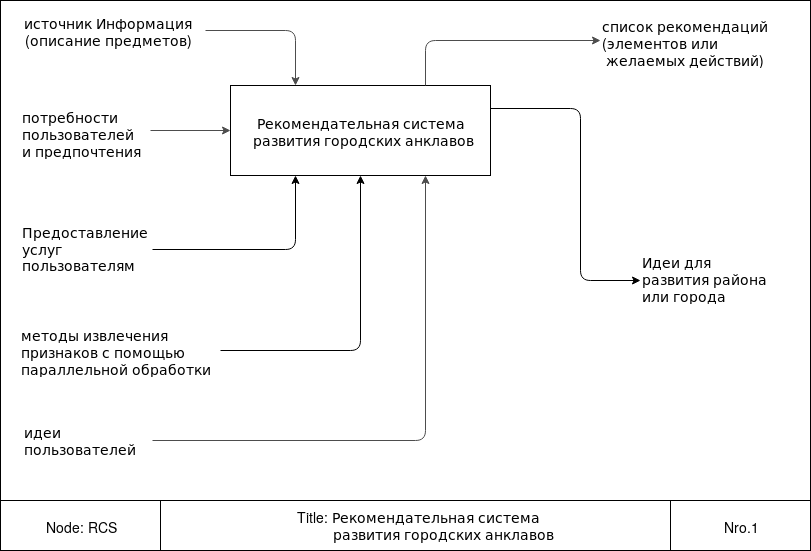
\includegraphics[scale=0.5]{diag1.png}
  \caption{Функциональная схема модели}
  \label{image:scheme3}
\end{figure}

\begin{figure}[h]
  \centering
  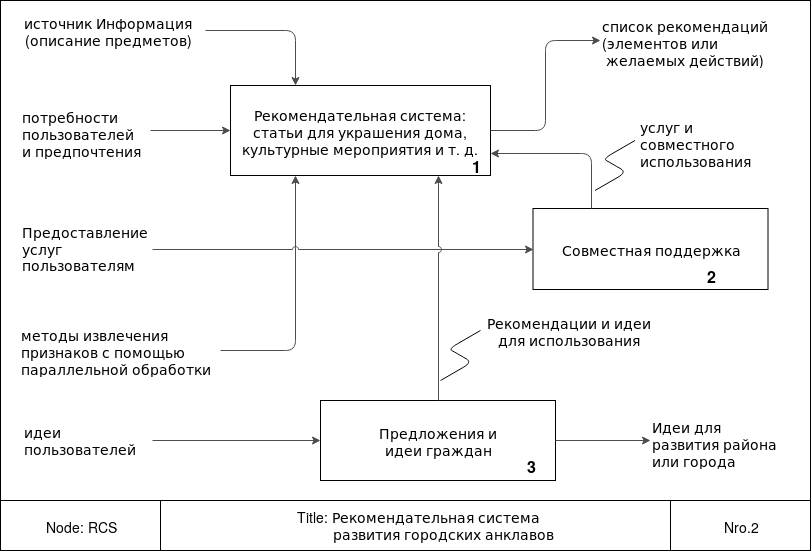
\includegraphics[scale=0.5]{diag2.png}
  \caption{Функциональная схема модели}
  \label{image:4}
\end{figure}
\hfill \break


\subsection{Лучшее использование отзывов пользователей}
Необходимо, чтобы люди получали рекомендации. Случай получения «ранжирования предметов» уже недостаточно. Кроме того, сайты рекомендаций не хотят делиться отзывами с третьими лицами. Система рекомендаций, которая управляет данными профиля пользователя, но может делиться отзывами с другими аналогичными системами с целью содействия сообществам.

Хорошо используемая обратная связь - это сила клиента, которая приносит пользу сообществу. С лучшей поддержкой мы будем стремиться содействовать развитию сообществ.

\begin{table}[]
\centering
\begin{tabular}{|p{2cm}|p{6cm}|p{6cm}|}
\hline
\multicolumn{3}{|p{14cm}|}{Классификация отзывов пользователей в соответствии с рекомендательными системами} \\ \hline
По релевантности       & Положительная информация (вывести характеристики, которые нравится пользователю).      &  Отрицательная информация (то есть выведение характеристик, которые не интересуют пользователя).      \\ \hline
Различные методы записи комментариев пользователей.       & Когда система требует, чтобы пользователь явно оценивал элементы, этот метод обычно известен как «явные комментарии».      &  Другой метод, называемый «неявной обратной связью», не требует активного участия пользователя в том смысле, что обратная связь получается из мониторинга и анализа действий пользователя.      \\ \hline
\end{tabular}
\centering
\caption{Feedback.}
\centering
\label{tabla:sencilla1}
\end{table}

\clearpage
\section{Рекомендательная Система}

Рекомендательная Система  - это система фильтрации информации \cite{recommender_system,filtering_system}, которая предоставляет пользователям ряд индивидуальных предложений о некоторых типах возможных предметов, которые они могут купить или выбрать. Задачей системы рекомендаций является преобразование данных и предпочтений пользователей в прогнозы возможных будущих вкусов и интересов пользователей. Индивидуальные рекомендации должны помочь вам выбрать правильный контент для нужного человека. 


\begin{figure}[h]
  \centering
  
\includegraphics[scale=0.5]{recommpeq2.png}
  \caption{Типовая схема рекомендательной системы}
  \label{image:}
\end{figure}


Электронная торговля на основе Рекомендальная система доминирует в розничной торговле. В «Рекомендационных системах» всем участникам выгодно, с одной стороны, продавцам разрешалось добираться до неизвестных клиентов через тесные отношения или один за другим, создавая лояльных покупателей через неявную помощь других покупателей, которые, бессознательно, являются ценной частью, предоставляет данные для рекомендации.

С другой стороны, клиент получает рекомендации и покупает то, что ему нужно, или то, что он считает нужным. В отрасли разрабатываются более эффективные алгоритмы, чтобы системы рекомендаций могли дать лучший и полезный список рекомендаций.

Теперь эта функциональность рекомендации покупки, как мы ее знаем, пересекает точку созревания, появятся новые алгоритмы, но необходим новый порядок рекомендаций, некоторые из них специфические и другие общие. Цель Рекомендальная система рекомендации в том, что благодаря своим предложениям отношения с клиентами создаются с помощью рекомендаций, а объем продаж максимизируется.

\begin{figure}[h]
  \centering
  
\includegraphics[scale=0.55]{celureco.png}
  \caption{Рекомендатор в ваших руках}
  \label{image:2}
\end{figure}
\newpage

\subsection{Необходимо указать на городские анклавы} Системы рекомендаций используются в электронной торговле, и им удалось монополизировать информацию: на сайте продаж есть вся информация о продуктах, содержании корзины, сделанных покупках и квалификации, которая будет служить для выработки рекомендаций. В обычном магазине это невозможно сделать, и это уменьшает объем продаж того же самого.

В этом новом мире, в котором нормальные магазины стремятся исчезнуть, отрасль стремится разработать все более совершенные алгоритмы для составления рекомендаций, чтобы максимизировать продажи в онлайн-сайтах.

Мы начнем определять систему рекомендаций прототипов, которая использует инструменты этой технологии, но с интересом к определенным группам пользователей, например, к пользователям, которые живут в определенном регионе или районе.

Эта «регионализация», в которой работает наша рекомендательная система, может занять каждый регион как «семью», где жители могут иметь одинаковые вкусы и потребности. В этой модели существуют области более развиты, то есть большее количество развлекательных и культурных мероприятий, мероприятий, которые полезны для улучшения внешнего вида окружающей среды (живопись, садоводство и т.д.), которые требуют продуктов, которые будут куплены или другие услуги типа " доля-экономика "\cite{shared_economy}.

Эти рекомендации могут также использоваться пользователями городских анклавов в целях их развития, принимая их в качестве примера, чтобы эволюционировать их окрестности. Но подумайте, можно ли свергнуть крупные интернет-сайты продаж? Ответ сегодня кажется нет, но правительства начинают обвинять монополистов в крупных сайтах онлайн-продаж, таких как Amazon. Возможно, что в какой-то момент они юридически ограничены для работы в глобальном масштабе или с большими налогами.

Электронная коммерция и запрограммированное устаревание \cite{planned_obsolescence} продуктов, заставляют потребителя повторять покупки, и именно там действуют традиционные системы рекомендаций. Желание покупать товары все быстрее и быстрее не делает людей счастливее.

Хотя невозможно предсказать будущее, если можно подготовиться к более совместной экономике, где рекомендуются не только продукты, но и общий опыт для развития. Система рекомендаций в совместной экономике могла бы:



\begin{enumerate}
\item Предлагайте экономическую экономию, позволяя узнать о интересах пользователей соседства и сотрудничать с предложениями о покупке групп.
\item Большее предложение для потребителя. Лучший доступ к другим альтернативам, которые до сих пор не были жизнеспособными или не были видны большинству из нас.
\item Устойчивое развитие. Совместная экономика поощряет и провоцирует второе использование продуктов.
\item Благоприятные эффекты для соревнований. Это способствует предпринимательству, стимулирует конкуренцию и экономическую активность. Они уже делят квартиры, транспортные средства, транспорт и т.д.
\item Социальная ценность. Содействие социальной сплоченности, солидарности и социальным отношениям, основанным на доверии. Вы можете создавать развлекательные и культурные мероприятия, присутствовать в других районах, но не существующих, в которых вы хотите улучшить.
\item Управление ресурсами. Использование ресурсов является еще одним из основных принципов совместной экономики, поскольку это то, что приносит пользу всем нам. Лучший пример - водитель, который делится своим автомобилем с несколькими пассажирами с близлежащими пунктами назначения.
\item Экологическая выгода. Сокращение производства с меньшими затратами природных ресурсов и меньшим загрязнением.
\end{enumerate}


Традиционные системы сотрудничества не поощряют разработку упомянутых тем, поскольку для них цель состоит в том, чтобы выработать более эффективные рекомендации относительно товаров для покупки.

\subsection{Используемая информация} 
Это применение характеризуется предоставлением рекомендаций пользователям автоматически, на основании уже совершенных действий (покупок, выставленных рейтингов, посещений и т.д.) и приемом от них обратной связи (заказы в магазинах, переход по ссылкам и т.п.).
Рекомендательные системы являются одним из важных разделов интеллектуального анализа данных - Data Mining.

Существует два типа квалификаций: явная и неявная квалификация. Явная квалификация - это те, которые пользователи сознательно и добровольно выразили в отношении предметов: «Мне это нравится», «они не так уж плохи» и «Мне это не нравится», или по рейтингам от 1 до 5, это позже совершить покупку и получить доступ к квалификации. Комментарии также являются плюсом и полезны на выборах.

Неявные оценки получаются при наблюдении за поведением пользователя. То, что пользователь нажимает на элемент, отражает некоторый интерес к нему, особенно если он добавлен в корзину покупок.

Даже принимая конкретный городской анклав, люди, которые ежедневно используют определенные услуги, такие как «собираются обедать или обедать», в какой-то ресторан в этом районе, могут квалифицироваться наиболее «широко»: в зависимости от контекста {обед, ужин} , {для работы, удовольствия}, также квалифицируют выбранное меню {в частности} и в соответствии со вкусом или типом приготовления. Даже частая частота одного и того же пользователя в определенном ресторане и запрос, например, «пицца», можно считать положительным.

В вышеупомянутом случае система рекомендаций в соответствии со всей собранной информацией может составить профиль пользователя, а затем рекомендовать другие близлежащие рестораны в соответствии с интересами, которые уже проявились. 



\subsection{Основные вызовы системы рекомендаций}

\begin{enumerate}
\item
Разнообразие данных. Когда среднее число оценок для каждого пользователя или элемента велико, они могут быть распределены неравномерно, и поэтому есть пользователи или элементы со многими оценками, а другие - с небольшим количеством. В случае предоставления локальных услуг его можно использовать как юниверс для близлежащих пользователей.

\item
Масштабируемость. По мере роста числа пользователей и предметов необходимо учитывать проблемы с вычислительными затратами и искать алгоритмы рекомендации, которые не требуют или не могут быть параллельными (или и теми и теми). Другим возможным решением является использование инкрементных версий алгоритмов, где, по мере роста информации, рекомендации не пересчитываются глобально, а постепенно.

\item
Холодный старт. Когда новый пользователь входит в систему, недостаточно информации для получения рекомендации для него. Хорошая система рекомендаций должна быть в состоянии справиться с этой ситуацией. Вот почему мы подчеркиваем, что, возможно, пользователи одного и того же региона могут иметь аналогичные предпочтения, которые помогают минимизировать холодный старт.

\item
Разнообразие по сравнению с точностью. Когда задача сосредоточена на рекомендации пунктов, которые могут быть оценены конкретным пользователем, обычно более эффективно рекомендовать элементы с высокими и популярными рейтингами. Хороший список рекомендуемых элементов также должен содержать менее очевидные элементы, которые пользователю сложнее выполнить самостоятельно.

\item
Уязвимость к атакам. Учитывая его важность в приложениях электронной коммерции, системы рекомендаций являются объектами атак для продвижения или подавления определенных предметов (этого было бы достаточно, чтобы создать ложные профили пользователей, с тем чтобы сделать положительную квалификацию для тех предметов, которые они хотели бы продвигать, и негативы для тех, кто хотел бы подавить ). Существует широкий набор инструментов, позволяющих избежать этих атак.

\item
начение времени. Есть предметы, которые интересуются только в течение определенного периода времени. Интересно знать, когда следует отклонять старые мнения и каковы временные шаблоны в оценках пользователей и актуальности предметов.

\item
Оценка рекомендаций. У нас есть разные показатели, но выбор лучшего для данной ситуации остается открытым. Сравнение между различными алгоритмами рекомендаций проблематично, потому что они решают разные задачи.

\item
Пользовательский интерфейс. Рекомендации должны быть прозрачными, чтобы пользователь знал, почему эти элементы были рекомендованы. Пользователю должен быть показан длинный список, но он представлен простым способом, и его легко ориентировать. В настоящее время интерфейс имеет очень большое значение, но считается, что в скором времени у нас будет мир без экранов \cite{screenless}, что приведет к усиленной реальности.

\item
Представьте себе, что в будущем системы рекомендаций будут основой стандарта для совершения покупок, но уже не с прокруткой списка пользователей, но одни и те же алгоритмы рекомендуют и совершают покупку. Например, холодильник может контролировать уровни существования пищи и делать заказы на покупку, когда они опускаются ниже определенного порога, выбирая, где покупать в соответствии с системой рекомендаций и совершая платеж через виртуальный кошелек.
\end{enumerate}


\subsection{Cтруктура}

Структура системы рекомендаций имеет форму двудольного графика, в котором на одном из подграфов представлены пользователи, а в других - элементы. Таким образом, дуги графа, которые соединяют пользователей с элементами, представляют собой квалификации между ними.


\begin{figure}[h]
  \centering
  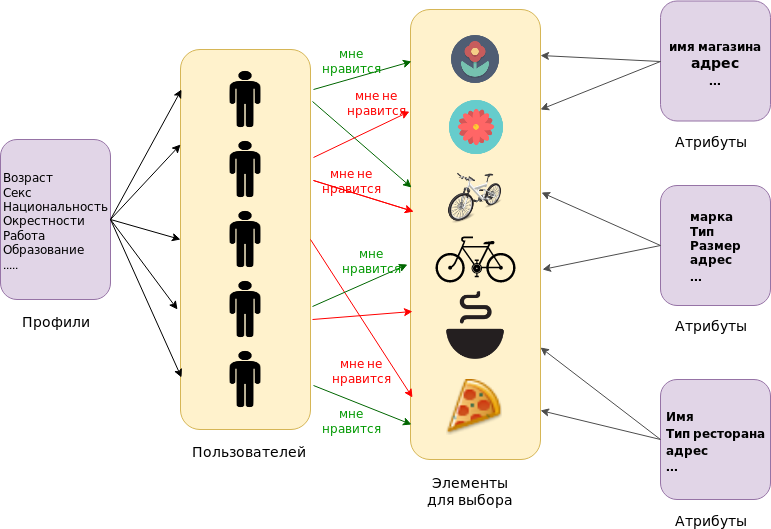
\includegraphics[scale=0.55]{struct_recomm.png}
  \caption{Структура системы рекомендаций}
  \label{image:scheme4}
\end{figure}

Проблема рекомендации может быть определена о том, как дать рекомендации пользователю о новых элементах на основе исторической информации, хранящейся в системе, и предложить этому пользователю новые и оригинальные элементы, для которых предсказанный ответ высок.

Тип ответов пользовательского элемента варьируется от одного приложения к другому и попадает в одну из этих четырех категорий: скалярный (1..5), текстовый (мне нравится, мне нравится, мне это не нравится, не согласен и т. д.), двоичный (мне нравится или мне это не нравится) и, наконец, унарный ответ, который захватывает взаимодействие пользователя с элементом (например, покупка, доступ в Интернет и т. д.) без предоставления явной информации об оценке пользователя для этого элемента.

Поскольку большинство пользователей склонны взаимодействовать с элементами, которые они находят интересными, унарные ответы по-прежнему предоставляют полезную информацию о предпочтениях пользователей.

«Сегодня люди любят оценивать и добавлять рекомендации, но возможно, что в ближайшем будущем унарный ответ может быть единственным признаком.»







